\documentclass[a4paper,12pt]{article}
\usepackage{graphicx}
\usepackage{float}
\usepackage{listings}
\usepackage{color}
\usepackage{courier}
\usepackage{geometry}
\geometry{margin=1in}
\usepackage{enumitem}
\usepackage{titlesec}

% Define Java syntax highlighting
\definecolor{javared}{rgb}{0.6,0,0}
\definecolor{javagreen}{rgb}{0.25,0.5,0.35}
\definecolor{javapurple}{rgb}{0.5,0,0.35}
\definecolor{javadocblue}{rgb}{0.25,0.35,0.75}
\lstset{
    language=Java,
    basicstyle=\ttfamily\small,
    keywordstyle=\color{javared}\bfseries,
    stringstyle=\color{javagreen},
    commentstyle=\color{javagreen}\itshape,
    morecomment=[s][\color{javadocblue}]{/**}{*/},
    numbers=left,
    numberstyle=\tiny\color{black},
    stepnumber=1,
    numbersep=10pt,
    tabsize=4,
    showspaces=false,
    showstringspaces=false
}

\newcommand{\practicaltitle}[1]{
    \newpage
    \begin{center}
        \Large\textbf{#1} \\
        \normalsize\vspace{0.5cm}
    \end{center}
}

\title{\textbf{Practical 1: Handling Various Data Types}}
% \practicaltitle{Practical 2: Another Java Topic}
\author{}
\date{}

% Redefine \subsection command to use hashtags instead of numbers
\titleformat{\subsection}[block]{\bfseries\large}{\texttt{\#}}{1em}{}

\begin{document}

\maketitle

\section{Introduction to Java}
JAVA was developed by James Gosling at Sun Microsystems Inc in May 1995 and later acquired by Oracle Corporation. It is a simple programming language. Java makes writing, compiling, and debugging programming easy. It helps to create reusable code and modular programs. Java is a class-based, object-oriented programming language and is designed to have as few implementation dependencies as possible. A general-purpose programming language made for developers to write once run anywhere that is compiled Java code can run on all platforms that support Java. Java applications are compiled to byte code that can run on any Java Virtual Machine. The syntax of Java is similar to C/C++.

Java is widely used for developing applications for desktop, web, and mobile devices. Java is known for its simplicity, robustness, and security features, making it a popular choice for enterprise-level applications.

\section{Java Syntax}
Java syntax is the set of rules defining how a Java program is written and interpreted.
\begin{figure}[h]
    \centering
    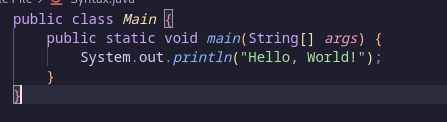
\includegraphics[width=0.8\linewidth]{images/basic_syntax.png}
    \caption{Basic Syntax of Java Program}
    \label{fig:sample_image}
\end{figure}

\subsection*{public class Main}
\begin{itemize}[leftmargin=2cm]
    \item \textbf{public}: An access modifier indicating that the class is accessible from other classes.
    \item \textbf{class}: A keyword used to define a class in Java.
    \item \textbf{Main}: The name of the class. By convention, class names in Java start with an uppercase letter.
\end{itemize}

\subsection*{public static void main(String[] args)}
\begin{itemize}[leftmargin=2cm]
    \item \textbf{static}: A keyword indicating that the method belongs to the class, not to instances of the class. It can be called without creating an object of the class.
    \item \textbf{void}:  The return type of the method, indicating that it does not return any value.
    \item \textbf{main}: The name of the method. This is the entry point of any Java application.
    \item \textbf{String[] args}: An array of String arguments passed to the method. These are command-line arguments.
\end{itemize}

\subsection*{System.out.println("Hello, World!")}
\begin{itemize}[leftmargin=2cm]
    \item \textbf{System}: A built-in class in the \texttt{java.lang} package.
    \item \textbf{out}: A static field in the \textbf{System} class, which is an instance of \textbf{PrintStream}.
    \item \textbf{println}: A method of \textbf{PrintStream} that prints a message to the standard output (usually the console) followed by a newline.
    \item \textbf{"Hello, World!"}: A string literal that is the message to be printed.
\end{itemize}


\section{Variables in Java}
Variables are containers for storing data values. In Java, every variable must be declared before it is used. A variable declaration includes the data type followed by the variable name. Java supports different types of variables, including:
\begin{itemize}[leftmargin=2cm]
    \item \textbf{Local Variables}: Declared inside a method and accessible only within that method.
    \item \textbf{Instance Variables}: Declared inside a class but outside any method. They are accessible from any method in the class.
    \item \textbf{Static Variables}: Declared with the \texttt{static} keyword. These are shared among all instances of the class.
\end{itemize}

\section{Data Types in Java}
Java has two categories of data types: \textbf{Primitive Data Types} and \textbf{Reference/Object Data Types}.

\subsection{Primitive Data Types}
Primitive data types are the most basic data types available in Java.
\begin{figure}[H]
    \centering
    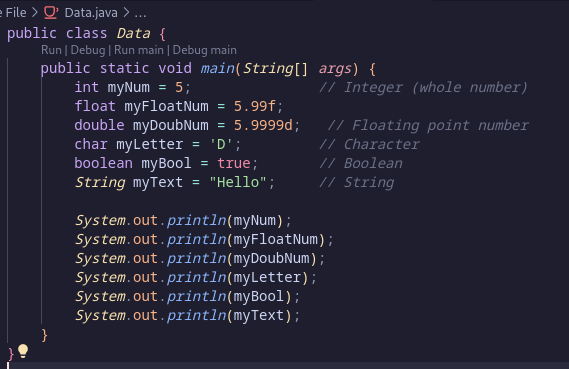
\includegraphics[width=0.9\linewidth]{images/DataType.png}
    \caption{Primitive Data types in Java}
    \label{fig:sample_image}
\end{figure}

\begin{itemize}[leftmargin=2cm]
    \item \textbf{byte}: 8-bit signed integer. Range: -128 to 127.
    \item \textbf{short}: 16-bit signed integer. Range: -32,768 to 32,767.
    \item \textbf{int}: 32-bit signed integer. Range: -2\textsuperscript{31} to 2\textsuperscript{31}-1.
    \item \textbf{long}: 64-bit signed integer. Range: -2\textsuperscript{63} to 2\textsuperscript{63}-1.
    \item \textbf{float}: 32-bit floating-point number.
    \item \textbf{double}: 64-bit floating-point number.
    \item \textbf{char}: 16-bit Unicode character.
    \item \textbf{boolean}: Represents two values: true and false.
\end{itemize}

\subsection{Non Primitive Data Types}
Reference types in Java are Strings and arrays:
\begin{figure}[H]
    \centering
    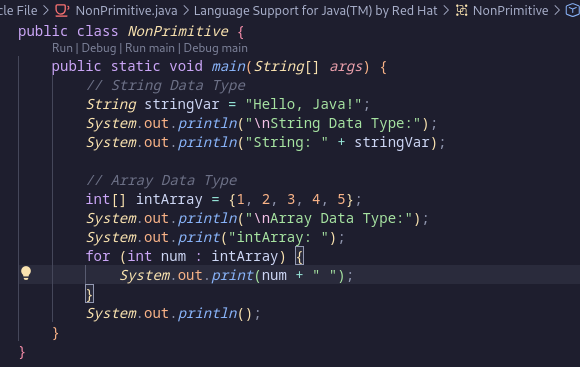
\includegraphics[width=0.9\linewidth]{images/non_primitve.png}
    \caption{Non-Primitive Data types in Java}
    \label{fig:sample_image}
\end{figure}

\begin{itemize}[leftmargin=2cm]
    \item \textbf{Strings}: Sequences of characters.
    \item \textbf{Arrays}: Containers that hold multiple values of the same type.
\end{itemize}

\setcounter{section}{0}

\practicaltitle{Practical 2: Type casting}
Type casting is when you assign a value of one primitive data type to another type. There are two types of type casting, implicit typecasting and explicit typecasting which are explained below: 

\section{Implicit Type Casting}
Implicit type casting is done automatically when passing a smaller size type to a larger size type.
\begin{center}
    \fbox{
        \parbox{0.9\linewidth}{
            \centering
            \texttt{byte $\rightarrow$ short $\rightarrow$ char $\rightarrow$ int $\rightarrow$ long $\rightarrow$ float $\rightarrow$ double}
        }
    }
\end{center}
\begin{figure}[H]
    \centering
    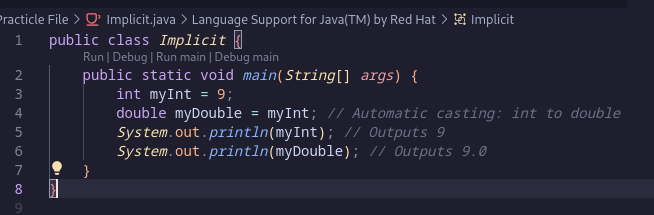
\includegraphics[width=0.9\linewidth]{images/implicit.png}
    \caption{Implicit Type Conversion}
    \label{fig:sample_image}
\end{figure}

\section{Explicit Type Casting}
Explicit type casting must be done manually by placing the type in parentheses () in front of the value.
\begin{center}
    \fbox{
        \parbox{0.9\linewidth}{
            \centering
            \texttt{double $\rightarrow$ float $\rightarrow$ long $\rightarrow$ int $\rightarrow$ char $\rightarrow$ short $\rightarrow$ byte}
        }
    }
\end{center}
\begin{figure}[H]
    \centering
    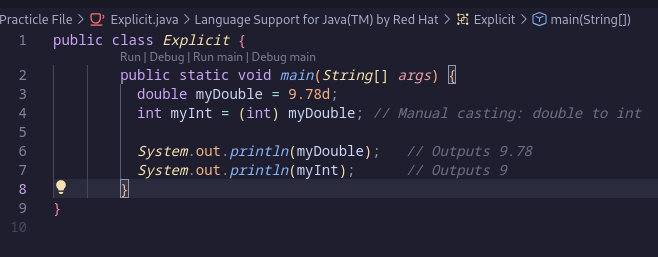
\includegraphics[width=0.9\linewidth]{images/explicit.png}
    \caption{Explicit Type Conversion}
    \label{fig:sample_image}
\end{figure}

\setcounter{section}{0}

\practicaltitle{Practical 3: Array 1D and 2D}

\section{1-Dimensional Array}
Arrays are used to store multiple values in a single variable, instead of declaring separate variables for each value.
\subsection{Code: }
\begin{figure}[H]
    \centering
    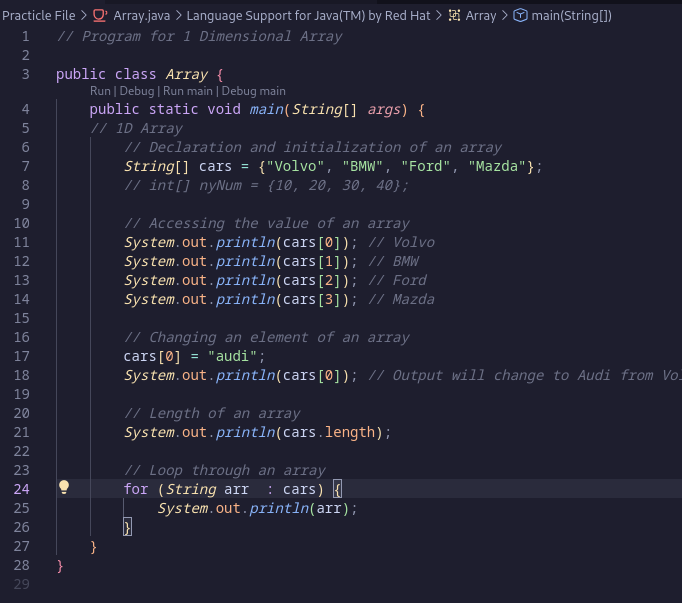
\includegraphics[width=0.8\linewidth]{images/array.png}
    \caption{1 Dimensional Array}
    \label{fig:sample_image}
\end{figure}
\subsection{Output: }
\begin{figure}[H]
    \centering
    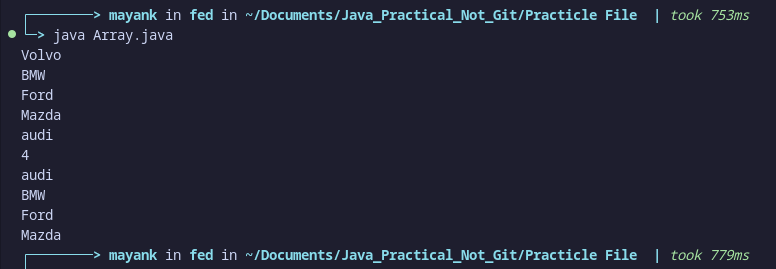
\includegraphics[width=0.9\linewidth]{images/output2.png}
    \caption{output of 1-D array}
    \label{fig:sample_image}
\end{figure}

\section{Multi Dimensional Array}
A multidimensional array is an array of arrays. Multidimensional arrays are useful when you want to store data as a tabular form, like a table with rows and columns.
\subsection{Code: }
\begin{figure}[H]
    \centering
    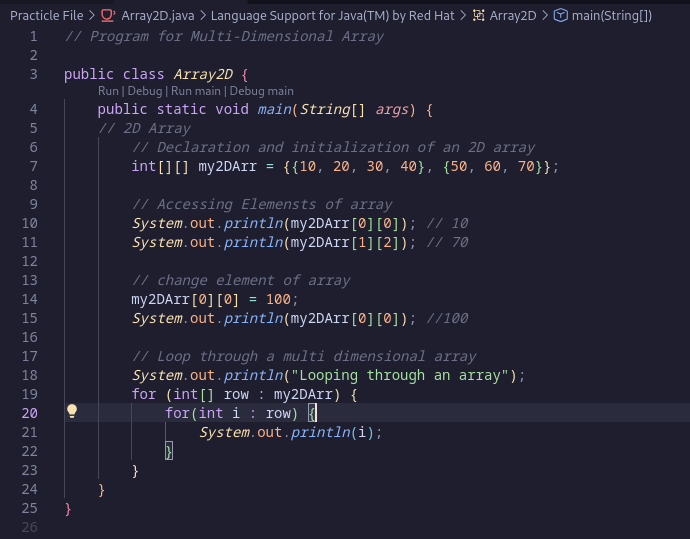
\includegraphics[width=0.8\linewidth]{images/array_2d.png}
    \caption{Multi Dimensional Array}
    \label{fig:sample_image}
\end{figure}
\subsection{Output: }
\begin{figure}[H]
    \centering
    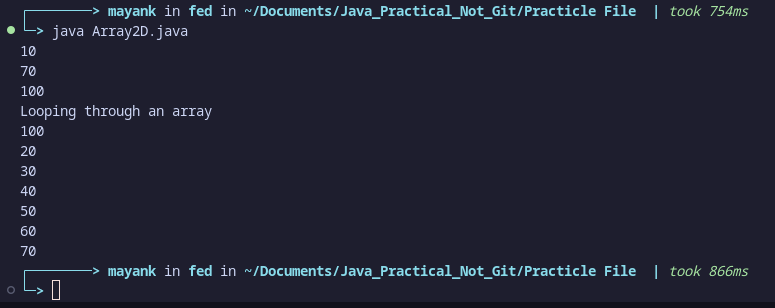
\includegraphics[width=0.9\linewidth]{images/output3.png}
    \caption{output of Multi-D array}
    \label{fig:sample_image}
\end{figure}

\setcounter{section}{0}

\practicaltitle{Practical 4: Various Control Strucutures}
In Java, control structures are constructs that dictate the order in which statements are executed in a program. They enable conditional execution, looping, and altering the normal sequential flow of control.


\section{The IF statement}
Use the if statement to specify a block of Java code to be executed if a condition is true.
\subsection{Code: }
\begin{figure}[H]
    \centering
    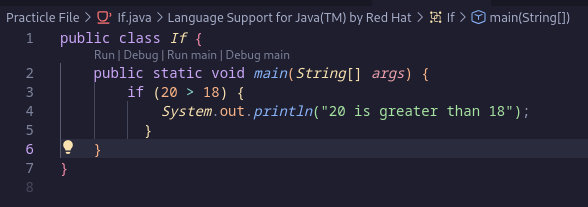
\includegraphics[width=0.9\linewidth]{images/if.png}
    \caption{if statement}
    \label{fig:sample_image}
\end{figure}
\subsection{Output: }
\begin{figure}[H]
    \centering
    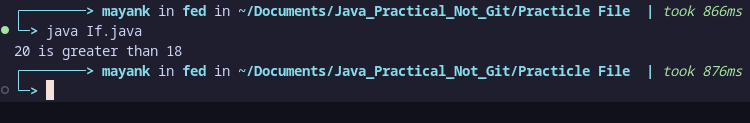
\includegraphics[width=0.9\linewidth]{images/output4.png}
    \caption{output of if statement}
    \label{fig:sample_image}
\end{figure}

\section{The IF-Else statement}
Executes one block of code if its condition evaluates to true, and another block of code if it evaluates to false.
\subsection{Code: }
\begin{figure}[H]
    \centering
    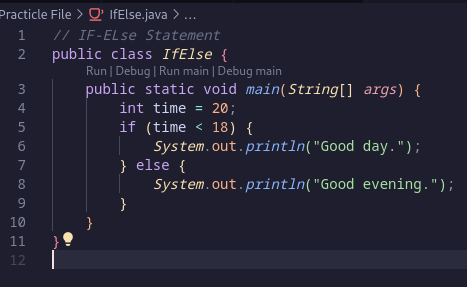
\includegraphics[width=0.9\linewidth]{images/if_else.png}
    \caption{if-else statement}
    \label{fig:sample_image}
\end{figure}
\subsection{Output: }
\begin{figure}[H]
    \centering
    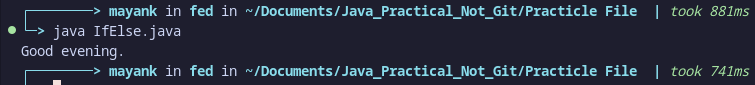
\includegraphics[width=0.9\linewidth]{images/output5.png}
    \caption{output of if-else statement}
    \label{fig:sample_image}
\end{figure}


\setcounter{section}{0}

\practicaltitle{Practical 4: Addition Of Two Numbers}
\section{Add Two Numbers by taking input from the user}
\subsection{Code: }
\begin{figure}[H]
    \centering
    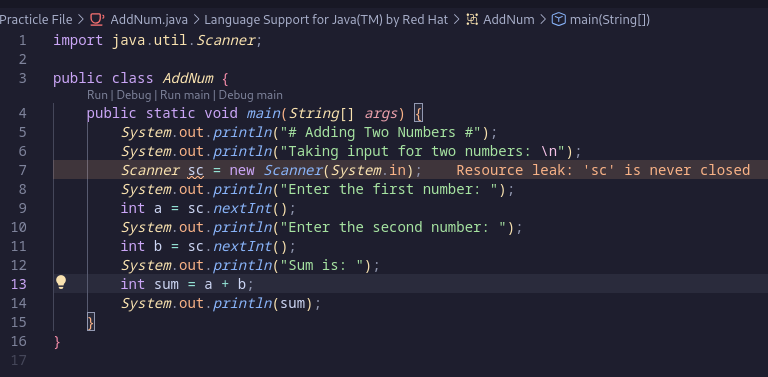
\includegraphics[width=0.9\linewidth]{images/add_num.png}
    \caption{Code of addition of two numbers}
    \label{fig:sample_image}
\end{figure}
\subsection{Output: }
\begin{figure}[H]
    \centering
    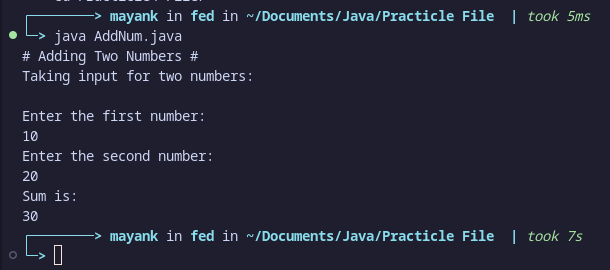
\includegraphics[width=0.9\linewidth]{images/output1.png}
    \caption{output of addition of two numbers}
    \label{fig:sample_image}
\end{figure}
\end{document}
